\clearpage
\raggedbottom
\section{Frozen replication and tail-misspecification experiments}\label{app:solid}

\subsection{Protocol and uncertainty}
A separately frozen protocol adds 630 sampling cells and 66 deterministic sensitivity configurations. All sampling cells use one NVIDIA H20, float64 particles, $G=64$, $d=8$, $U=20$, $\kappa=1$, the same quadratic time grid, and systematic resampling below an ESS fraction of $0.5$. Configuration order is randomized before execution. Sampler times are synchronized GPU wall times for the sampling loop, including subset selection and diagnostic logging, and excluding reference integration, model prediction, certificate computation, and file packaging. Three preliminary smoke cells are excluded from all reported statistics.

The learned-density replication crosses the five fixed final checkpoints with 20 new dataset seeds, 100--119. At $K=2048$, $P=32768$, and $M=4$, each of these 100 pairs is evaluated with full weighting, raw unbiased without-replacement weighting, and tail control without replacement, giving 300 cells. No checkpoint, dataset, or method is selected using the new results. We report mean marginal W1 against both the learned composition and the true posterior. Percentile intervals use 10,000 bootstrap draws, independently resampling the five training seeds and 20 dataset seeds on each draw while preserving method pairing. These intervals describe the limited training/data ensemble; the 100 pairs do not constitute 100 independent training replicates. The artifacts also retain the five per-training-seed means and intervals conditional on the fixed checkpoints.

The boundary study uses the three oracle families, $K\in\{512,2048\}$, $P=8192$, and ten new sampling seeds, 20--29. It compares full weighting, raw without-replacement weighting at $M_{\rm crit}-1$ and $M_{\rm crit}$, and tail control at $M=4$, giving 240 cells. Here $M_{\rm crit}$ is the previously reported first certified finite batch size, independently rechecked before sampling. The final 90 cells keep the target fixed and replace the component variance in the affine control by $\widetilde v_g=(1+\delta)v_g$, with $\delta\in\{-0.1,0,0.1\}$, $K=512$, $P=8192$, $M=4$, and sampling with replacement. Control means are unchanged. This is a common multiplicative variance perturbation across factors and coordinates, not an arbitrary score-error model. Oracle intervals resample the ten sampling seeds with method pairing.

The deterministic sensitivity grid uses both time resolutions and
\[
 \delta\in\{-0.25,-0.1,-0.05,-0.025,-0.01,0,0.01,0.025,0.05,0.1,0.25\}.
\]
Proposition~\ref{prop:control} supplies the constant-batch certificate for these misspecified affine controls. The exact-tail case $\delta=0$ agrees with full weighting in its quadratic coefficients. For nonzero $\delta$, the estimator remains conditionally unbiased, but its strict integrability domain must be checked again.

\subsection{Replication on new learned-density compositions}
Full weighting and tail control are finite in all 100 new checkpoint/dataset pairs each; raw without-replacement weighting is infinite in all 100 pairs. Table~\ref{tab:solid-heldout} and Figure~\ref{fig:solid-heldout} report the complete comparison. The paired tail-minus-full W1 difference is $0.08042$, with a crossed-bootstrap 95\% interval of $[0.07028,0.09052]$. The five training-seed means of this difference range from $0.07759$ to $0.08390$. Against the true posterior, the paired difference is $0.07929$ with interval $[0.06900,0.08953]$. The larger tail-control error therefore persists on the new datasets and across the existing training seeds.

\begin{table}[H]
 \centering
 \caption{New learned-density replication: means and crossed-bootstrap 95\% intervals over five fixed checkpoints and 20 new datasets. W1 is mean marginal Wasserstein distance. Times are mean H20 sampler seconds. The last column reports finite certificates out of 100 pairs.}
 \label{tab:solid-heldout}
 \small
 \begin{tabular}{lccrr}
 \toprule
 Method & W1 to learned & W1 to true & Seconds & Finite\\
 \midrule
 Full & $0.01817\ [0.01634,0.02036]$ & $0.01985\ [0.01723,0.02319]$ & 14.06 & 100\\
 Raw WOR & $0.04725\ [0.04252,0.05240]$ & $0.04776\ [0.04308,0.05285]$ & 2.97 & 0\\
 Tail WOR & $0.09859\ [0.08831,0.10878]$ & $0.09914\ [0.08836,0.10950]$ & 3.40 & 100\\
 \bottomrule
 \end{tabular}
\end{table}

Tail control takes about $24.2\%$ of the sampler time of full weighting on this hardware and configuration, but its mean W1 to the learned composition is about $5.43$ times as large. This is a fixed-particle, fixed-grid comparison, not a matched-accuracy speedup. All five networks are reused without further training, and their predictions are computed once per dataset; these timings do not represent repeated neural score evaluations.

\begin{figure}[H]
 \centering
 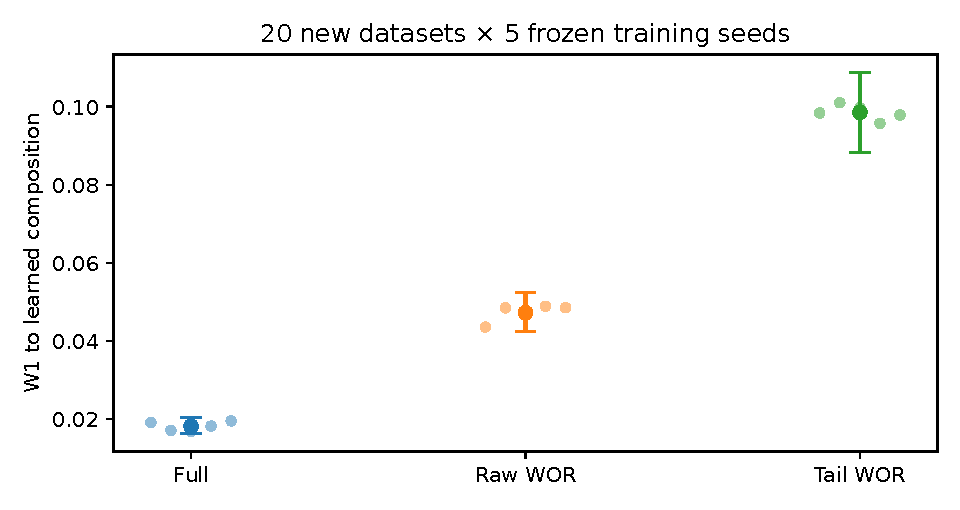
\includegraphics[width=0.82\linewidth]{figures/solid_heldout.pdf}
 \caption{New learned-density replication. Large points show overall means with crossed-bootstrap 95\% intervals; five smaller points show the means for individual training seeds, each averaged over the same 20 datasets. Raw WOR has an infinite population normalizer throughout, whereas Full and Tail WOR are finite throughout.}
 \label{fig:solid-heldout}
\end{figure}

\subsection{Sampling on both sides of a validity threshold}
The rechecked critical batch sizes are 60 and 59 for the Gaussian and ordinary-mixture families at $K=512$ and 2048, respectively, and 18 and 17 for the weak mixture. In each of these six settings, the certificate is infinite at $M_{\rm crit}-1$ and finite at $M_{\rm crit}$. Both full weighting and $M=4$ tail control are finite. Table~\ref{tab:solid-boundary} includes every setting, with intervals in Figure~\ref{fig:solid-boundary}.

\begin{table}[H]
 \centering
 \caption{Mean marginal W1 across ten new sampling seeds near the certificate boundary. Below and At use raw WOR with $M=M_{\rm crit}-1$ and $M=M_{\rm crit}$, respectively. Below is infinite in every row; the other three conditions are finite. Tail uses $M=4$.}
 \label{tab:solid-boundary}
 \begin{tabular}{lrrrrrr}
 \toprule
 Family & $K$ & $M_{\rm crit}$ & Full & Below & At & Tail\\
 \midrule
 Gaussian & 512 & 60 & 0.01854 & 0.02385 & 0.01543 & 0.01911\\
 Gaussian & 2048 & 59 & 0.01965 & 0.01777 & 0.02172 & 0.02107\\
 Mixture & 512 & 60 & 0.86302 & 0.81897 & 0.68900 & 1.43500\\
 Mixture & 2048 & 59 & 0.85092 & 0.85712 & 0.66242 & 1.52086\\
 Weak mixture & 512 & 18 & 0.04455 & 0.03798 & 0.03498 & 0.03523\\
 Weak mixture & 2048 & 17 & 0.02948 & 0.03142 & 0.03945 & 0.03397\\
 \bottomrule
 \end{tabular}
\end{table}

Observed accuracy changes in both directions across the validity boundary. For the ordinary mixture at $K=2048$, the At-minus-Below difference is $-0.19469$, with paired interval $[-0.33562,-0.05965]$. For the weak mixture at the same resolution, it is $0.00802$, with interval $[0.00061,0.01784]$. These are descriptive intervals without adjustment across the six boundary comparisons. The certificate classifies existence of the population update; it does not require a monotone change in finite-particle endpoint error at the threshold.

\begin{figure}[H]
 \centering
 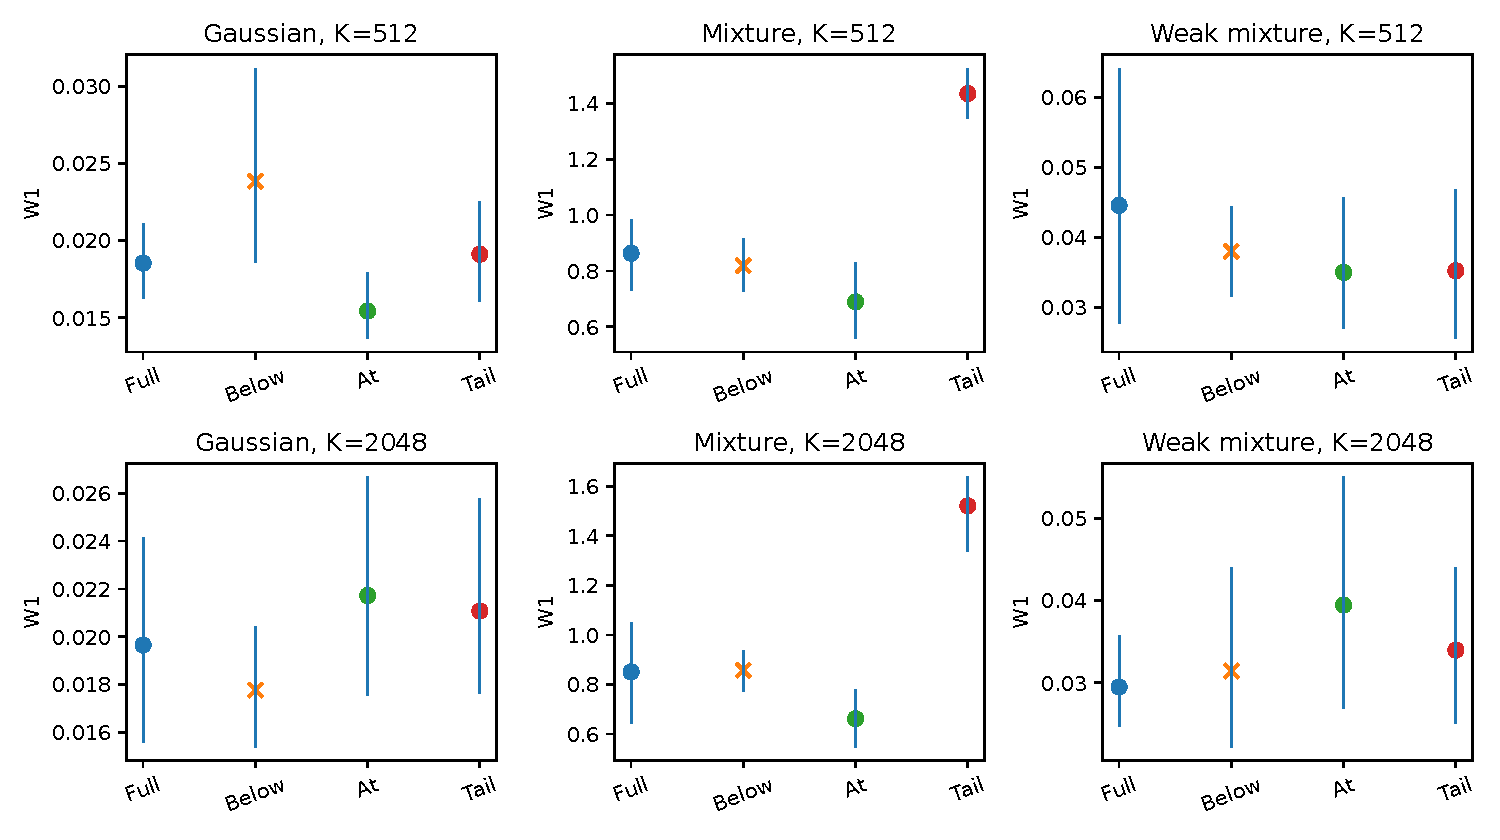
\includegraphics[width=\linewidth]{figures/solid_boundary.pdf}
 \caption{All six boundary comparisons, each with ten sampling seeds. Points show means and vertical bars show bootstrap 95\% intervals. Circles denote finite normalizers and crosses infinite ones. Panel-specific vertical scales retain the differences in error magnitude between families.}
 \label{fig:solid-boundary}
\end{figure}

\subsection{Sensitivity to an imperfect tail control}
Figure~\ref{fig:solid-tail-sensitivity} reports all 66 deterministic perturbations. Every tested perturbation with $|\delta|\le0.1$ is finite for all three families and both grids. At $\delta=\pm0.25$, the Gaussian and ordinary-mixture certificates are infinite on both grids, whereas the weak-mixture certificates remain finite. There are 58 finite and eight infinite configurations; no zero-denominator case is classified. These grid values demonstrate tolerance to the specified perturbations in the tested models, without establishing a uniform robustness interval for arbitrary factors or score errors.

\begin{table}[H]
 \centering
 \caption{Mean marginal W1 under multiplicative control-variance error, with the target held fixed. Each entry averages ten seeds at $K=512$, $P=8192$, $M=4$, with replacement. Every displayed setting has a finite certificate.}
 \label{tab:solid-tail-error}
 \begin{tabular}{lrrr}
 \toprule
 Family & $\delta=-0.1$ & $\delta=0$ & $\delta=0.1$\\
 \midrule
 Gaussian & 0.01974 & 0.01845 & 0.01882\\
 Mixture & 1.14131 & 1.18388 & 1.35780\\
 Weak mixture & 0.03086 & 0.03385 & 0.03260\\
 \bottomrule
 \end{tabular}
\end{table}

Finite certificates do not eliminate sensitivity of sampling error. For the ordinary mixture, the $\delta=0.1$ minus $\delta=0$ difference is $0.17392$, with a descriptive paired interval of $[0.00940,0.36340]$. The complete seed-level results and all six perturbation-comparison intervals are retained, including intervals spanning zero.

\begin{figure}[H]
 \centering
 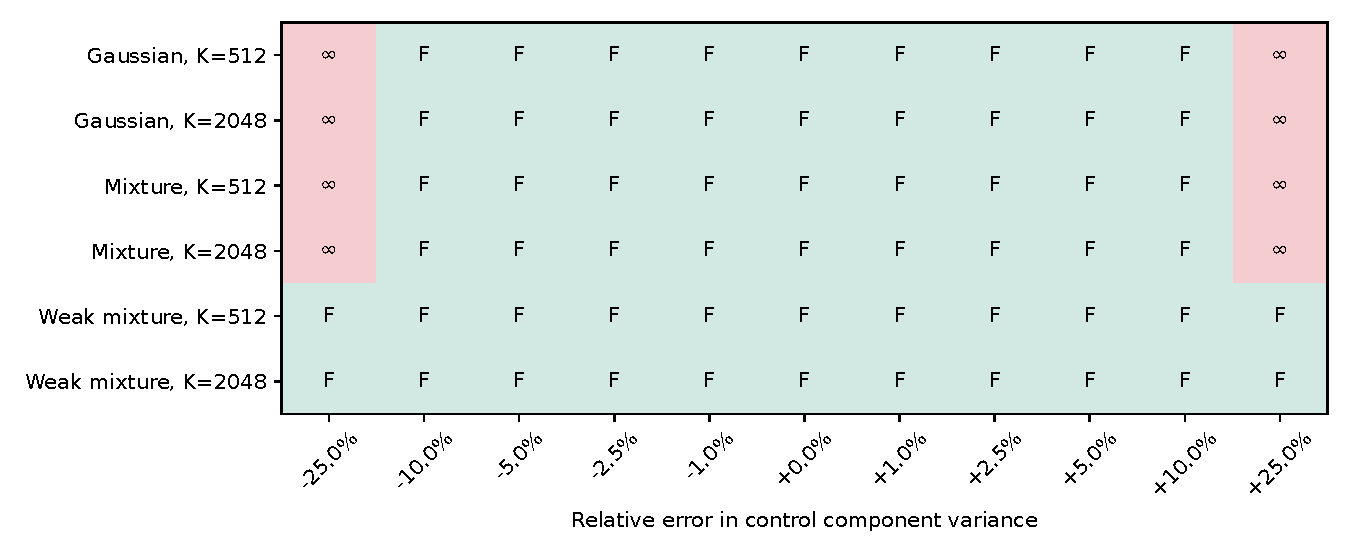
\includegraphics[width=\linewidth]{figures/solid_tail_sensitivity.pdf}
 \caption{Strict-domain certificates for every tested control-variance perturbation. F denotes a finite normalizer and $\infty$ an infinite one. Columns are the discrete tested values of $\delta$, not a continuous parameter grid or an assertion about untested values.}
 \label{fig:solid-tail-sensitivity}
\end{figure}

\subsection{Independent verification and remaining scope}
All 630 sampling cells completed with a zero launcher exit status, and every original particle array is retained. We reload all five checkpoints, regenerate the 20 datasets, and verify the 100 learned parameter sets and their consistency across methods. Independent SciPy reference calculations use 131,073 points on $[-16,16]$, with a separately implemented Gaussian-mixture density. These checks cover 103 learned/oracle parameter settings and their corresponding true-posterior references. Independent recomputation checks W1, KS, means, variances, and positive-coordinate masses for every cell. The maximum W1 discrepancy against the original records is $1.61\times10^{-6}$. A separate vectorized recursion checks 333 sampling-certificate configurations and all 66 sensitivity configurations, including failure steps. Source hashes, checkpoint hashes, complete cell manifests, and the recovered raw-file hashes are retained.

This replication strengthens evidence within the controlled simulator and explicit Gaussian-tail model class. It introduces no additional training replicates and provides no validation on a real scientific inverse problem, arbitrary neural scores, or non-diagonal tails. The new data support the distinction between population validity and finite-particle accuracy; they do not establish general speed--accuracy superiority for tail control.
